% set font and paper size
\documentclass[11pt,a4paper]{article}

% change to german
\usepackage[german]{babel}

% better hyphenation
\usepackage[final]{microtype}
\usepackage{csquotes}

% packages, images, math
\usepackage{geometry, graphicx, amsmath, amsfonts, array, multicol, multirow}

% bar charts
\usepackage{bchart}

% for bibliography
\usepackage[
    backend=biber,
    style=alphabetic,
    sorting=ynt,
    minalphanames=3,
]{biblatex}
\addbibresource{./res/references.bib}

% remove dots in ToC
\usepackage{tocloft}

% import line spacing
\usepackage{setspace}

% listings
\usepackage{listings}

% colors
\usepackage{xcolor}

% spacing between section titles and text
\usepackage{titlesec}
\titlespacing*{\section}{0pt}{0.7ex}{0.7ex}
\titlespacing*{\subsection}{0pt}{0.7ex}{0.7ex}
\titlespacing*{\subsubsection}{0pt}{0.7ex}{0.7ex}

% for urls
% break urls on line end
\usepackage[breaklinks, colorlinks=true, urlcolor=gray, citecolor=gray, linkcolor=black]{hyperref}

% Remove Indentation at new line
\setlength{\parindent}{0cm}

% Set Font to Arial, needs xelatex
\usepackage{unicode-math}
\usepackage{fontspec}
\setmainfont{Arial}

% Set Layout
\geometry{
    a4paper,
    left=25mm,
    right=25mm,
    top=25mm,
    bottom=20mm
}

% plots
\usepackage{pgfplotstable}
% recommended:
\usepackage{booktabs}
\usepackage{array}
\usepackage{colortbl}

\usepackage{pgfplots}

% moving in tikz picture
\usepackage{changepage}

% position figures
\usepackage{float}

% b tree
\usepackage{tikz}
\usetikzlibrary{shapes, arrows}

% set line spacing
\setstretch{1.5}

% remove ToC page number
\AtBeginDocument{\addtocontents{toc}{\protect\thispagestyle{empty}}} 

% bold caption
\usepackage[labelfont=bf]{caption}

% document
\begin{document}

% deckblatt
% title
\title{Schwierigkeiten bei Implementierung und Evaluation von Datenstrukturen in Datenbanksystemen}
\author{Anton Rodenwald (19)}
\maketitle

% page settings
\addtocounter{page}{-3}
\thispagestyle{empty}

\large
\begin{tabular}{l p{12cm}}

    Fachgebiet:          & Mathematik/Informatik   \\

    Wettbewerbssparte:   & Jugend Forscht          \\

    Bundesland:          & Niedersachsen           \\

    Wettbewerbsjahr:     & 2024                    \\

    Thema des Projektes: &
    In meinem Projekt wollte ich verschiedene in Datenbanksystemen genutzte Datenstrukturen
    implementieren und testen. Dabei betrachtete ich auch unterschiedliche Ansätze der
    Datenspeicherung und für den Datenzugriff. Bei den auftretenden Schwierigkeiten
    musste ich Lösungen finden und adaptieren.     \\

    Projektbetreuerin:   & Birgit Ziegenmeyer      \\

    Institution:         & Schillerschule Hannover \\
\end{tabular}

\clearpage

\pagestyle{empty}

% kurzfassung

\section*{Kurzfassung}

In meinem Projekt wollte ich erforschen, wie die in Datenbanksystemen genutzten
Datenstrukturen die Zugriffsgeschwindigkeit beeinflussen und welche Datenstrukturen
sich für welche Arten von Daten besonders gut eignen.
Dazu wollte ich ein Datenbanksystem in C++ entwickeln und messen, wie
schnell, je nach Datenstruktur, auf die Daten zugegriffen werden kann.
Die Haupt-Schwierigkeit war dabei allerdings die hohe Komplexität,
weshalb ich nur einige Datenstrukturen umsetzen und testen konnte.
Insgesamt lässt sich feststellen, dass noch weitere Messungen nötig
sind, um die Ergebnisse zu konsolidieren.
Dies lässt noch viele weitere Möglichkeiten für weitere Forschungen zu.

\clearpage

% inhaltsverzeichnis

\renewcommand*\contentsname{Inhaltsverzeichnis}

% \renewcommand{\cftdot}{}

\tableofcontents

\clearpage

\pagestyle{plain}

\section{Einleitung}

\subsection{Motivation}

Im Rahmen des Informatik-Leistungkurses meiner Schule haben wir (Mitschüler und ich) uns
mit Datenbanken und Daten-Modellierung beschäftigt. Da jedoch auf die Funktionsweise einer
Datenbank nicht weiter eingegangen wurde und ich auch schon von unterschiedlichen
Datenbankansätzen, genauer Relationalen und Nicht-Relationalen, gehört hatte,
wollte ich mich im Rahmen meines Projektes genauer damit beschäftigen
und mehr darüber lernen.
Nachdem ich einen spannenden Vortrag von Richard Hipp gesehen hatte,
entschied ich mich, dass ich selbst eine Datenbank umsetzen wollte \cite{sql_ideas}.

\subsection{Forschungsfrage}

Meine Forschungsfrage ist, wie die Wahl der Datenstruktur die
Geschwindigkeit einer Datenbank beeinflusst und inwiefern sich eine Datenstruktur
für gewisse Daten besser oder schlechter eignet.

\subsection{Ziel}

Mein ursprüngliches Ziel war die Entwicklung einer Datenbank
mit den Datenstrukturen R-Tree, B-Tree, Binary-Tree und Graphen.
Davon konnte ich leider aufgrund der hohen Komplexität (stand jetzt) nur ein
Binäres-Such-Array und eine Graph-Datenstruktur umsetzen.

\clearpage

\section{Hintergrund}

\subsection{Arten von Daten und Datenstrukturen}

Verschiedene Datenarten sind dabei räumliche, zeitliche, relationale
(als Objekte modellierbare) und stark vernetzte Daten
\cite{no_sql_wikipedia} \cite{indian_overview}.

\vspace*{0.3cm}

Räumliche Daten sind z. B. Kartendaten (Google Maps, OpenStreetMap). Bestimmte Landmarken oder Objekte
(Bäume, Mulleimer) lassen sich beispielsweise als Punkte auf einer Fläche modellieren.
Es müssen dann effizient Fragen wie z. B. ``Wie viele Mülleimer gibt es in diesem Park?'' oder ``Was sind
die 3 am besten bewerteten Restaurants in der Innenstadt?'' beantwortet werden.
Eine dafür ausgelegte Datenstruktur ist der R-Tree.

\vspace*{0.3cm}

Zeitliche Daten können z. B. die von einem Sensor gemessenen Temperaturen sein.
Wichtig wäre bei diesen, dass sich statistische Größen wie Durchschnittswerte einfach
bilden lassen und Anomalien erkannt werden.

\vspace*{0.3cm}

Daten, die klassischerweise in relationalens Datenbanken gespeichert werden,
lassen sich als Objekte modellieren.
Beispielsweise speichert ein Unternehmen über Kunden immer die gleichen Daten
(Name, E-Mail, ...). Jeder Datensatz kann dann eindeutig z. B. über eine
ID identifiziert werden. Eine dafür geeignete Datenstruktur ist der B-Tree, eine
dem Binary-Tree ähnliche Datenstruktur.

\vspace*{0.3cm}

Wenn zwischen einzelnen Daten von z. B. jedem Nutzer einer Social-Media-Plattform
allerdings viele Beziehungen bestehen (Follower, Likes), so eignet sich eine
Graph-Datenstruktur besser. Diese ermöglicht dann, schnell die Verbindungen
zwischen Nutzern herausfinden, um z. B. Gruppen innerhalb des Netzwerks zu erkennen.

\subsection{Arten von Datenbanksystemen}

Moderne Datenbanksysteme ermöglichen meist, mit einem System verschiedene
Speicherungsformen zu nutzen. Trotzdem muss man sich bei einem Multi-Modalen System
natürlich überlegen, welche Daten man nun in welcher Art von Datenstruktur speichern
möchte. Die Website \href{https://db-engines.com/en/ranking}{db-engines.com} stellt z. B.
eine Übersicht über die aktuell beliebtesten Datenbanksysteme und deren Modalitäten dar.

\section{Vorgehen}

\subsection{Schwierigkeiten bei der Implementierung}

Mein geplantes Vorgehen bestand darin, ein Datenbanksystem mit diesen
verschiedenen Datenstrukturen in C++ umzusetzen.
Während des Entwicklungsprozesses und der Implementierung zeigte sich allerdings die
zunehmende Komplexität, weswegen ich nur begrenzt die verschiedenen Datenstrukturen
vergleichen konnte. Trotzdem werde ich die angestrebten Datenstrukturen
zumindest in ihrer Funktion erläutern und meine Schwierigkeiten bei der Umsetzung
beschreiben.
Auch werde ich meine dann tatsächlich durchgeführten Tests beschreiben.
Also ein ganz normaler Entwicklungsprozess nach dem Zitat:

\begin{quote}
    \guillemetright we do these things not because they are easy, \\
    \hspace*{0.2em} but because we thought they were going to be easy\guillemetleft
\end{quote}

Zu Beginn meines Projektes setzte ich auch
die Kommunikation über Linux Websockets um, da Datenbanksysteme
eine Schnittstelle zu anderen Programmen benötigen.
Da mein Datenbank-Backend allerdings nicht rechtzeitig ausgereift genug war, konnte
ich diese Schnittstelle noch nicht in Kombination mit dem Rest testen.
(Code auf \href{https://github.com/Redstonerayy/light-db}{Github})

\subsection{Testdaten}

Bei den Testdaten handelt es sich um eine fiktive Schülerschaft, in der jeder
Schüler Freundschaften und Feindschaften hat. Diese Testdaten generierte ich mir
mit einem Python Script und speicherte diese in einer CSV-Datei.
Jeder Schüler hat dabei eine ID und einen Namen, der eine zufällige Zeichenkette ist.
Anschließend sind bei jedem Schüler noch 100 Freund- und Feindschaften eingetragen.
Jede dieser Beziehungen wird dabei durch die ID eines anderen Schülers beschrieben.
Schüler $0$ ist z. B. mit Schüler $255777$ befreundet.

\begin{lstlisting}
0, eszycidpyopumzgd, 255777-14862-..., 204372-226894-...
1, idixqgtnahamebxf, 233658-369416-..., 265451-355559-...
2, digztyrwpvlifrgj, 104446-129174-..., 188986-42660-...
...
\end{lstlisting}

% \clearpage

\subsection{Teststruktur}

Bei meinen Performance Tests verglich ich die Suchgeschwindigkeit der Datenstrukturen.
Die gleichen Testdaten wurden in beide Datenstrukturen eingelesen und anschließend
wurde gemessen, wie schnell auf einen bestimmten Teil der Daten jeweils zugegriffen
werden kann. Im 1. Test sollten alle Freunde von Schüler Nr. 2 und im 2. Test alle
Feindschaften von Schüler Nr. 1 gefunden werden.

\subsection{Probleme bei B-Tree und Binary-Tree}

Da der B-Tree eine in vielen Datenbanken verwendete Datenstruktur ist, wollte ich
diesen zuerst implementieren. Als Grundlage nahm ich die erste B-Trees beschreibende
Veröffentlichung von 2 Boeing-Entwicklern \cite{boeing_engineers}.

\vspace*{0.3cm}

Der B-Tree ist dabei ähnlich zu einem binären Suchbaum.
Der Hauptunterschied ist, dass jeder Node mehr als nur 2 Child-Nodes
hat, wodurch der Baum weniger tief ist.
Um Elemente zu suchen, zu löschen oder zu ändern folgt man, ähnlich wie beim
Binary-Tree, der Baumstruktur vom Root Node ausgehend.
Durch Vergleiche innerhalb der Nodes und das Traversieren der
Äste findet man ein bestimmtes Element oder eine Position im Baum.

\begin{figure}[H]
    \begin{center}
        \begin{tikzpicture}
            \tikzstyle{bplus}=[rectangle split, rectangle split horizontal,rectangle split ignore empty parts,draw]
            \tikzstyle{every node}=[bplus]
            \tikzstyle{level 1}=[sibling distance=80mm]
            \tikzstyle{level 2}=[sibling distance=15mm]
            \node {15} [->]
            child {node {3 \nodepart{two} 7}
                    child {node {1 \nodepart{two} 2}}
                    child {node {4 \nodepart{two} 6}}
                    child {node {8 \nodepart{two} 9}}
                }
            child {node {21 \nodepart{two} 28 \nodepart{three} 32 \nodepart{four} 50}
                    child[sibling distance=20mm] {node {17 \nodepart{two} 20}}
                    child[sibling distance=20mm] {node {22 \nodepart{two} 25}}
                    child[sibling distance=20mm] {node {28 \nodepart{two} 30}}
                    child[sibling distance=25mm] {node {34 \nodepart{two} 38 \nodepart{three} 44 \nodepart{four} 47}}
                    child[sibling distance=30mm] {node {53 \nodepart{two} 54 \nodepart{three} 60 \nodepart{four} 88}}
                }
            ;\end{tikzpicture}
    \end{center}
    \caption{\textbf{B-Tree der Tiefe 2}}
\end{figure}

Bei der Implementierung des B-Tree traten allerdings einige Probleme auf.
Das größte Problem war, dass die Ausbalancierung beim B-Tree relativ komplex ist.
Deshalb entschied ich mich dafür, andere Datenstrukturen zu testen.
Auch entschied ich mich, meine Tests ausschließlich mit im RAM liegenden Daten
durchzuführen, da eine Speicherung auf einer Festplatte noch mehr Komplexität bedeutet
hätte. Da der R-Tree eine modifizierte Version des B-Tree ist, konnte ich auch diesen
somit nicht umsetzen.

\vspace*{0.5cm}

Anschließend implementierte ich als Alternative dann einen AVL-Tree, eine sich selbst
ausbalancierende Variante des binären Suchbaums. Beim anschließenden
Konzeptionieren der Performance-Tests entdeckte ich allerdings noch einen
beim Einfügen von Elementen auftretenden Fehler bei meinem AVL-Tree,
weswegen ich mich spontan dazu entscheiden musste, auch diesen nicht zu testen.

\subsection{Such-Array}

Aufgrund der vorigen Schwierigkeiten testete ich nun nicht
mit einem B-Tree oder Binary-Tree, sondern wandte die binäre Suche
auf ein sortiertes Array an. Prinzipiell nutzen aber alle 3 Datenstrukturen die
binäre Suche. Deswegen nahm ich an, dass alle 3 Datenstrukturen bei Daten im RAM
ähnlich schnell Daten finden können.
Die Testdaten sind in diesem Fall auf 3 Such-Arrays (vgl. Tabellen)
aufgeteilt, jeweils eine für Schüler, Freundschaften und Feindschaften.

\begin{table}[H]
    \centering
    \begin{tabular}{|l|l|}
        \hline
        Schüler\_1\_ID & Schüler\_2\_ID \\ \hline
        5              & 7              \\ \hline
        5              & 75             \\ \hline
        5              & 456            \\ \hline
        5              & 45             \\ \hline
    \end{tabular}
    \qquad
    \begin{tabular}{|l|l|}
        \hline
        Schüler\_1\_ID & Schüler\_2\_ID \\ \hline
        7              & 629            \\ \hline
        7              & 762            \\ \hline
        7              & 229            \\ \hline
        7              & 29435          \\ \hline
    \end{tabular}
    \caption{\textbf{Tabellenausschnitte Freundschaften/Feindschaften}}
\end{table}

Um alle Freunde/Feinde eines Schülers zu finden, müssen in
den als Assoziationstabellen fungierenden, sortierten Such-Arrays
alle Datensätze zwischen dem kleinstmöglichen und größtmöglichen Wert
gefunden werten. Beispielsweise für den Schüler $5$ alles zwischen (inklusiv) den Datensätzen
$5 | 0$ und $5 | m$ wenn $m$ die Anzahl an Schülern ist. Da das Such-Array
nach beiden Spalten sortiert ist, muss nur mit der binären Suche das linke
und das rechte Ende des Bereichs bestimmt werden. Anschließend können in linearer
Zeit alle gesuchten Datensätze ausgelesen werden.

% \vspace*{0.5cm}

\begin{figure}[H]
    \centering
    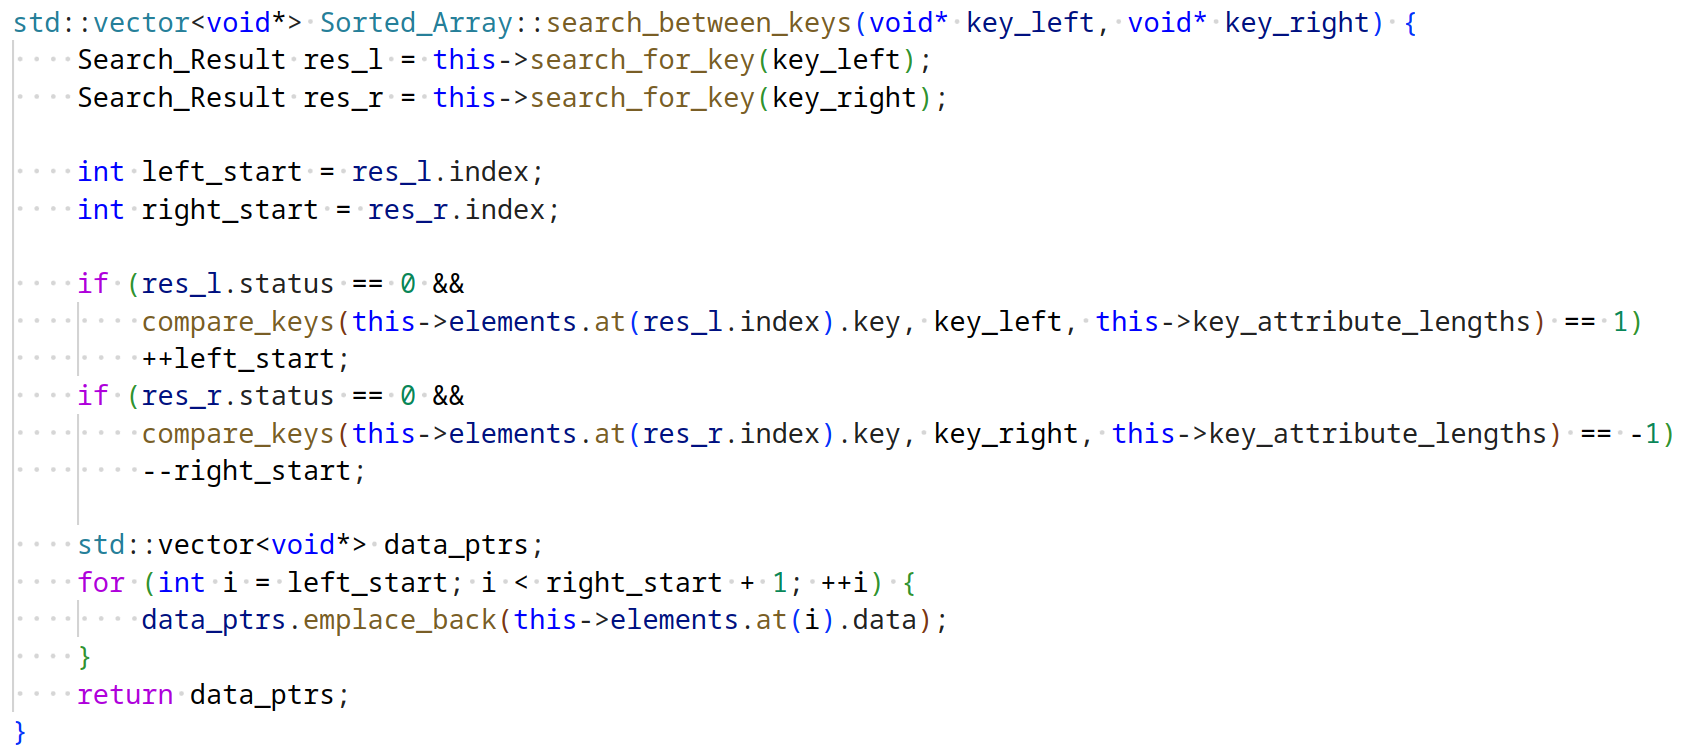
\includegraphics[width=1.1\textwidth]{./res/code_sort_array.png}
    \caption{\textbf{C++ Code der Such-Array Suchfunktion}}
\end{figure}

\subsection{Graph-Datenstruktur}

Bei meiner Implementierung einer Graph-Datenstruktur sind in jedem Node
die Daten und die Verbindungen zu anderen Nodes gespeichert.
Um alle Freundschaften oder Feindschaften zu erhalten, muss nur über diese
Daten iteriert werden und man erhält schnell die Daten der befreundeten oder
befeindeten Schüler. Die Art der Verbindung (Freund/Feind) kann dabei durch
das $link\_schema$ festgelegt werden.

\begin{figure}[H]
    \centering
    \begin{tikzpicture}[->,>=stealth',shorten >=1pt,auto,node distance=3cm,
            thick,main node/.style={circle,draw,font=\sffamily\Large\bfseries}]

        \node[main node] (1) {1};
        \node[main node] (2) [below left of=1] {2};
        \node[main node] (3) [below right of=1] {3};

        \path[every node/.style={font=\sffamily\small}]
        (1) edge [bend right] node[left] {Freund} (2)
        (2) edge node [right] {Freund} (1)
        edge node {Feind} (3)
        (3) edge [bend right] node[right] {Feind} (1);
    \end{tikzpicture}
    \caption{\textbf{Graph mit Beziehungen zwischen Schülern}}
\end{figure}

\vspace*{0.5cm}

\begin{figure}[H]
    \centering
    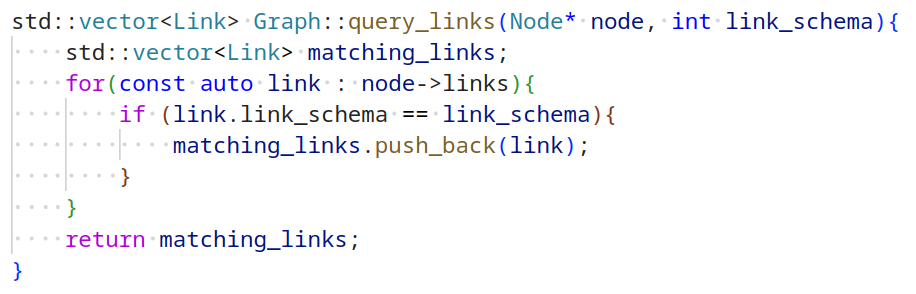
\includegraphics[width=1.0\textwidth]{./res/code_graphdb.png}
    \caption{\textbf{C++ Code der Graph-Suchfunktion}}
\end{figure}

\subsection{Komplexitäts Analyse}

\begin{align*}
    & f_g = \text{Anzahl Freundschaften} \quad
    F_g = \text{Anzahl Feindschaften} \\ 
    & f = \text{Anzahl Freunde eines Schülers} \quad
    F = \text{Anzahl Feinde eines Schülers} \\
    & s = \text{Anzahl Schüler} \quad
\end{align*}

Beim Such-Array muss mit der binären Suche jeweils die linke und rechte Begrenzung
ermittelt werden. Anschließend müssen alle Freunde bzw. Feinde des
Schülers durchlaufen werden.

\begin{equation*}
    O(2 \cdot ( log_2(f_g) + 1 ) + f)
\end{equation*}

Bei der Graph-Datenstruktur müssen alle Verbindungen durchlaufen werden, also
die Summe der Vebindungen aus Freund- und Feindschaften.

\begin{equation*}
    O(f + F)
\end{equation*}

Anhand der Komplexitäten lässt sich erwarten, dass die Graph-Datenstruktur deutlich
schneller ist.

\section{Messwerte}

Meine Messungen führte ich auf meinem Desktop-PC und meinem Laptop (Plugged-In) durch.
Auf jedem Computer nahm ich 2 Messreihen auf.
Jede der 4 Anfragen an die 2 Datenstrukturen wurde jeweils 50-mal direkt hintereinander
ausgeführt.
$SA$ beschreibt die Datenstruktur Such-Array. $G$ steht für Graph-Datenstruktur.
Das $F$ beschreibt die Suche nach allen Freunden des Schülers Nr. 2.
Das $H$ beschreibt die Suche nach allen Feindschaften (Hostilities) des Schülers Nr. 1.

\vspace*{1cm}

\begin{figure}[H]
    \centering
    \begin{tikzpicture}[scale=1]
        \begin{axis}[
                x label style={at={(axis description cs:0.5,-0.01)},anchor=north},
                y label style={at={(axis description cs:-0.01,0.5)},anchor=south},
                xlabel=\textbf{Nummer der Messung},
                ylabel=\textbf{Zeit in Nanosekunden},
                width=1.0\textwidth,
                height=0.7\textwidth,
            ]
            \addplot table [y=$SA_F$, x=NR]{./res/data_pc_1.dat};
            \addlegendentry{$SA_F$ series}
            \addplot table [y=$SA_H$, x=NR]{./res/data_pc_1.dat};
            \addlegendentry{$SA_H$ series}
            \addplot table [y=$G_F$, x=NR]{./res/data_pc_1.dat};
            \addlegendentry{$G_F$ series}
            \addplot table [y=$G_H$, x=NR]{./res/data_pc_1.dat};
            \addlegendentry{$G_H$ series}
        \end{axis}
    \end{tikzpicture}
    \vspace*{-0.8cm}
    \caption{\textbf{1. Messreihe am PC (Ryzen 7 2700)}}
\end{figure}

\begin{figure}[H]
    \centering
    \begin{tikzpicture}[scale=1]
        \begin{axis}[
                x label style={at={(axis description cs:0.5,-0.01)},anchor=north},
                y label style={at={(axis description cs:-0.01,0.5)},anchor=south},
                xlabel=\textbf{Nummer der Messung},
                ylabel=\textbf{Zeit in Nanosekunden},
                width=1.0\textwidth,
                height=0.7\textwidth,
            ]
            \addplot table [y=$SA_F$, x=NR]{./res/data_pc_2.dat};
            \addlegendentry{$SA_F$ series}
            \addplot table [y=$SA_H$, x=NR]{./res/data_pc_2.dat};
            \addlegendentry{$SA_H$ series}
            \addplot table [y=$G_F$, x=NR]{./res/data_pc_2.dat};
            \addlegendentry{$G_F$ series}
            \addplot table [y=$G_H$, x=NR]{./res/data_pc_2.dat};
            \addlegendentry{$G_H$ series}
        \end{axis}
    \end{tikzpicture}
    \vspace*{-0.8cm}
    \caption{\textbf{2. Messreihe am PC (Ryzen 7 2700)}}
\end{figure}

\begin{figure}[H]
    \centering
    \begin{tikzpicture}[scale=1]
        \begin{axis}[
                x label style={at={(axis description cs:0.5,-0.01)},anchor=north},
                y label style={at={(axis description cs:-0.01,0.5)},anchor=south},
                xlabel=\textbf{Nummer der Messung},
                ylabel=\textbf{Zeit in Nanosekunden},
                scaled ticks=false,
                width=1.0\textwidth,
                height=0.7\textwidth,
            ]
            \addplot table [y=$SA_F$, x=NR]{./res/data_laptop_1.dat};
            \addlegendentry{$SA_F$ series}
            \addplot table [y=$SA_H$, x=NR]{./res/data_laptop_1.dat};
            \addlegendentry{$SA_H$ series}
            \addplot table [y=$G_F$, x=NR]{./res/data_laptop_1.dat};
            \addlegendentry{$G_F$ series}
            \addplot table [y=$G_H$, x=NR]{./res/data_laptop_1.dat};
            \addlegendentry{$G_H$ series}
        \end{axis}
    \end{tikzpicture}
    \vspace*{-0.8cm}
    \caption{\textbf{1. Messreihe am Laptop (Ryzen 5 5500U)}}
\end{figure}

\begin{figure}[H]
    \centering
    \begin{tikzpicture}[scale=1]
        \begin{axis}[
                x label style={at={(axis description cs:0.5,-0.01)},anchor=north},
                y label style={at={(axis description cs:-0.01,0.5)},anchor=south},
                xlabel=\textbf{Nummer der Messung},
                ylabel=\textbf{Zeit in Nanosekunden},
                scaled ticks=false,
                width=1.0\textwidth,
                height=0.7\textwidth,
            ]
            \addplot table [y=$SA_F$, x=NR]{./res/data_laptop_2.dat};
            \addlegendentry{$SA_F$ series}
            \addplot table [y=$SA_H$, x=NR]{./res/data_laptop_2.dat};
            \addlegendentry{$SA_H$ series}
            \addplot table [y=$G_F$, x=NR]{./res/data_laptop_2.dat};
            \addlegendentry{$G_F$ series}
            \addplot table [y=$G_H$, x=NR]{./res/data_laptop_2.dat};
            \addlegendentry{$G_H$ series}
        \end{axis}
    \end{tikzpicture}
    \vspace*{-0.8cm}
    \caption{\textbf{2. Messreihe am Laptop (Ryzen 5 5500U)}}
\end{figure}

\section{Deutung der Messwerte}

Bei den Messwerten am PC lässt sich erkennen, dass in den ersten paar Messungen die
benötigte Zeit deutlich höher ist als bei den restlichen, nachfolgenden Messungen.
Die benötigte Zeit aller Tests pendelt sich auf einem niedrigeren Niveau ein.
Gleiches ist auch am Laptop zu beobachten, wo die Messpunkte jedoch unregelmäßiger sind.
Dies lässt sich vermutlich auf eine Speicherung von Werten im CPU-Cache zurückführen,
in dem nach den ersten Durchläufen Daten vorgehalten werden, was zu besseren
Messergebnissen führt.
Vereinzelt gibt es auch in diesen Bereichen bei PC und Laptop ausreißende Werte.
Diese sind wahrscheinlich Mess-Anomalien, erzeugt durch einmalige Lastspitzen.
Diese könnten durch andere Prozesse auf dem Testsystem oder durch hardwarebedingte 
Faktoren verursacht worden sein.
Betrachtet man die 1. Messung, wo die Werte noch auseinanderliegen,
so lässt sich nicht feststellen, dass keine der Datenstrukturen schneller
ist als die anderen. Interessant ist bei diesen ersten Messwerten, dass die Messungen
bei gleich strukturierten Daten (Freundschaften und Feindschaften) deutlich voneinander
Abweichen. Auch für gleiche Datenstrukturen gibt es große Abweichungen der
benötigten Zeit.
Nicht überraschend sind die abweichenden Niveaus von PC und Laptop,
da bei CPUs mit unterschiedlichem Leistungsniveau logischerweise auch andere
Performance-Werte erzeugt werden.
Als dies lässt darauf schließen, dass es wahrscheinlich noch
unbekannte Faktoren gibt, die die Performance oder Messung beeinflussen.
Durch Identifizieren und Eliminieren dieser ließen sich vermutlich noch
genauere und aussagekräftigere Messwerte gewinnen.

\section{Beantwortung der Forschungsfrage}

Abschließend lässt sich die Forschungsfrage insofern beantworten, als dass
die Wahl der Datenstruktur in diesem Fall keinen Einfluss auf die Zugriffsgeschwindigkeit
hat. Keine der Datenstrukturen scheint der anderen überlegen, zumindest auf Basis
der Messwerte.

\section{Schwierigkeiten und Limitationen}

Bei der Umsetzung der Datenbank und den Tests hatte ich einige Probleme.
Eine Sache, die ich nicht prüfen konnte ist, wie sich der Speicherort der Daten
auswirkt. Also inwiefern Cache, RAM und Art des Massenspeichers (HDD, SSD)
sich auf die Geschwindigkeit beim Datenzugriff auswirken.
Dazu wollte ich eigentlich \href{https://www.amd.com/en/developer/uprof.html}{AMDuProf}
nutzen, eine von AMD für Ryzen CPUs bereitgestellte Software, mit der sich tiefgreifende
Daten über die Arbeit der CPU sammeln lassen. Mit dieser hätte ich z. B. Cache-Misses
der CPU analysieren können, doch leider lief diese nicht auf meinem System.
Auch konnte ich nicht prüfen, welche Anfragen an eine Datenbank CPU limitiert
und welche I/O bzw. Netzwerk limitiert sind. Dies war leider deswegen nicht
möglich, weil ich noch kein vollständiges Datenbanksystem hatte.

\section{Fazit}

Insgesamt konnte ich nicht so viele relevante Daten sammeln, würde das Projekt aber
trotzdem als lehrreich bewerten. Mir persönlich hat es einen guten Einblick in
Datenbanken und andere interessante Themen wie Socket-Programmierung gegeben
und ich konnte mehr über Datenstrukturen, C/C++ und gdb (GNU Debugger) lernen.

\clearpage

% break urls
\emergencystretch=0.5em

\section{Quellenangaben}

\section*{Links}

\url{https://github.com/Redstonerayy/light-db}

\url{https://beej.us/guide/bgnet/html/}

\url{https://db-engines.com/en/ranking}

\url{https://www.amd.com/en/developer/uprof.html}

\printbibliography[title={Literaturverzeichnis}]

\end{document}
